\documentclass{my_paper}
\usepackage{ctex}
\usepackage[textwidth=444bp,vmargin=2.5cm]{geometry}%设置页边距
\usepackage{array} %主要是增加列样式选项
\usepackage[dvipsnames]{xcolor}%颜色宏包
\usepackage{graphicx}%图片宏包
\usepackage{amsmath}%公式宏包
\usepackage[T1]{fontenc}    
\usepackage{newtxtext, newtxmath}  %两种使用Times New Roman 字体的方法
\usepackage{subfigure}
\usepackage{tabularx, booktabs} %% Load packages that you use
\usepackage{multirow} %跨行处理
\usepackage{rotating}%横向表格
\usepackage{diagbox}%斜线划分表头

\usepackage { gensymb }
% 打°符号\degree
\usepackage{framed}
\usepackage{listings}
% 代码
\usepackage{color} %red, green, blue, yellow, cyan, magenta, black, white
\usepackage[numbered,framed]{matlab-prettifier}%matlab 代码高亮
\usepackage{mdframed}%另一个边框
% matlab代码样式,使用方法为:
% \lstinputlisting[style=Matlab-editor,linewidth=\textwidth]{code.m}
% 或:
% \begin{lstlisting}[style=matlab-prettifier]
%     %code
% \end{lstlisting}
\renewenvironment{framed}[1][\hsize]
  {\MakeFramed{\hsize#1\advance\hsize-\width \FrameRestore}}%
  {\endMakeFramed}
%   修正framed环境,使之可以变长,用法:
%   \begin{framed}[1.2/textwidth]...

\usepackage{hologo}
\usepackage{gbt7714}
\bibliographystyle{gbt7714-numerical}
% 采用国标参考文献引用
\newcommand{\lunwenbiaoti}{\fontsize{15.75pt}{0}\heiti 基于熵权法的中小微企业银行信贷模型}
\newcommand{\zhaiyao}{\fontsize{14pt}{0}\heiti 摘要}
    
\begin{document}

\lstdefinestyle{python_style}{
 columns=fixed,
 numbers=left,                                        % 在左侧显示行号
 numberstyle=\tiny\color{gray},                       % 设定行号格式
 frame=trbl,                                        % 单线背景边框
 breaklines=true,                                     % 设定LaTeX对过长的代码行进行自动换行
 keywordstyle=\color[RGB]{40,40,255},                 % 设定关键字颜色
 numberstyle=\footnotesize\color{darkgray},
 commentstyle=\it\color[RGB]{0,96,96},                % 设置代码注释的格式
 stringstyle=\rmfamily\slshape\color[RGB]{128,0,0},   % 设置字符串格式
 showstringspaces=false,                              % 不显示字符串中的空格
 language=python,                                        % 设置语言
 basicstyle=\linespread{1.0}\fontsize{10bp}{10bp}\selectfont\ttfamily,                      % 字体字号
 %lineskip=10bp,
 %baselinestretch=1,
}
\newpage
\begin{center}
\lunwenbiaoti

\vspace{2ex}
\zhaiyao
\end{center}

基于中小企业规模小,资金不足的特点,银行依据中小企业的经营状况,给出贷款策略。本文首先利用多元线性回归的方法,以利润率等五个指标作为自变量,建立了还款能力评估模型,随后利用熵权法建立贷款数量界定模型,最后使用多目标规划法,平衡收益和用户流失,确定了企业贷款利率。除此之外,使用K近邻算法对缺失信誉等级进行补充,并针对新冠疫情带来的突发影响,引入系数进行调整。

针对问题一,为了解决银行的放贷问题,我们将问题化解为向谁贷款,贷款数目,贷款利率三个子问题。基于多变量线性回归建立企业还款能力评估模型,依据熵权法建立贷款数量分配模型,根据多目标规划建立了最优的利率设置,分别解决了提出的三个问题。使用的方法基于利润率,有效交易占比,供应链丰富度,信誉等级,平均单价,资金缺口六个要素,丰富全面挖掘了附件的信息。

针对问题二,我们在信誉等级缺失的情况下,利用K近邻算法预测附件二中的信誉等级。随后使用问题一所建立的银行借贷模型进行贷款分配。

针对问题三,面对新冠疫情等可能的突发因素影响,我们对银行信贷模型做出调整。首先搜寻相关资料,通过企业名称来推断企业所处类别,随后整理不同行业下受新冠影响的程度。最后对模型中利润率和资金缺口两项进行调整,做到了针对不同行业的企业都有对应策略。

该模型建立在较多的资料收集和数据分析基础上,客观可靠,具有较好的推广性。

\begin{guanjianci}
 元胞自动机 \quad 边缘检测 \quad 形状匹配
\end{guanjianci}

%----------- 正文 ----------
%----------- 一、问题重述 ----------
\newpage
\section{一、问题重述}

\subsection{问题背景}

为了给予中小企业现金支持,银行针对中小企业的特点,推出一系列不同的信用贷款。对于实力较强信用较好的企业,银行倾向于提供更加优惠的利率。我们需要针对小微企业的开票情况,建立数学模型来给出银行的信贷策略。


\subsection{问题重述}
经过分析整理,我们需要解决以下问题:
\begin{enumerate}
    \item 对附件1给出有信贷记录的123家企业的信贷风险进行量化分¬析,给出该银行在年度信贷总额固定时对这些企业的信贷策略。
    \item 在问题1的基础上,对附件2中没有信贷记录的302家企业的信贷风险进行量化分析,并给出该银行在年度信贷总额为1亿元时对这些企业的信贷策略。
    \item 综合考虑附件2中各企业的信贷风险和可能的突发因素(例如:新冠病毒疫情)对各企业的影响,给出该银行在年度信贷总额为1亿元时的信贷调整策略。
\end{enumerate}

\section{二、问题分析}
\subsection{问题一的分析}

为了解决问题1,需要利用附件中的小微企业发票数据和信誉评级来构建数学模型,以给出银行在年信贷额固定时的信贷策略。因此,我们利用企业发票数据估计营业额,资金缺口和稳定情况,且结合信用评级来给出信贷策略。因此,我们需要构建模型以解决贷款给谁、贷款多少以及利率多少的问题。

\subsection{问题二的分析}
为了解决问题2,需要对问题一中提出的银行信贷模型进行补充。由于不知道企业的信誉评级,我们可以利用附件一中已知的数据,构建KNN等机器学习算法,对缺失的用户标签进行预测。随后利用银行信贷模型组织信贷分配。

\subsection{问题三的分析}
为了能够定量地呈现出突发情况下银行地信贷调整策略,我们先按照企业的名称将企业进行行业分类。然后以新冠疫情为例,搜集疫情对各行业地影响程度和方面,然后将这些影响带入到响应自变量中,重新组织和实现之前的信贷策略模型。

%----------- 三、模型假设 ----------
\section{三、模型假设}
%使用代码片段:、jiashe%
\begin{enumerate}
    \item 假设企业发票明细完整无误,没有瞒报漏报。
    
    \textbf{原因:}依据企业的发票开具情况,可以直观显示出一个企业的收入支出。因此通过完整的发票记录,可以得到企业的经营特点。

    \item 假设企业都在同一时间办理信贷业务。
    
    \textbf{原因:}
    为了简化模型,做出此假设后可以灵活分配银行的贷款资金。且在实际生活中,银行在工作日都有资金流动,可以将一年期的信贷行为统一处理。

    \item 各企业经济特征不会有较大变化。
    
    \textbf{原因:}我们的模型是建立在已有数据基础之上的,有一定程度的“预测性”,若想要获得较好的“预测结果”,我们需要数据具有一定的“保持性”。

    \item 企业名称符合一般的起名习惯。
    
    \textbf{原因:}
    我们在对企业做行业划分时,是根据企业名称进行的,所以需要企业在名称中体现企业的行业属性。

    \item 企业仅从事一方面经营。
    
    \textbf{原因:}
    题目中的企业都为中小企业,很难具备多项业务同时处理的能力,同时不考虑复合型企业,也可以简化模型,提高模型的效率。

    
\end{enumerate}

%----------- 四、符号说明 ----------
\section{四、符号说明}
%使用三线表格最好~

\subsection{符号说明}
以下是本文使用的符号以及含义:
\begin{table}[h]%htbp表示的意思是latex会尽量满足排在前面的浮动格式,就是h-t-b-p这个顺序,让排版的效果尽量好。
    \centering
    \begin{tabular}{p{2.0cm}<{\centering}p{9.0cm}<{\centering}p{2.0cm}<{\centering}}
 %指定单元格宽度, 并且水平居中。
    \hline
    符号 & 说明 & 单位 \\ %换行 
    \hline
    $x_1$ & 利润率 &  元\\
    $x_2$ & 有效交易占比 &  /\\
    $x_3$ & 供应链丰富度 &  /\\
    $x_4$ & 信誉等级 &  /\\
    $x_5$ & 平均单价 &  元\\
    $x_6$ & 资金缺口 &  元\\
    $T,t$ & 发票集合,单张发票金额 &  /\\
    $P$ & 企业还款概率 &  /\\
    $C$ & 贷款额度 &  元\\
    $I$ & 贷款利率 &  元/年\\
    $R$ & 信贷收益 &  元\\
    $L$ & 流失率 &  /\\
    
    \hline
    \end{tabular}
\end{table}

%----------- 五、模型的建立与求解 ----------
\newpage
\section{五、模型的建立与求解}

以下将对提出的三个问题进行建模求解。
\subsection{基于熵权法的银行信贷模型}
银行信贷的过程主要是解决三个问题:贷给谁,贷多少钱以及贷款利率多少。针对借贷对象而言,需要评估其还款能力来做出贷款选择,我们将在5.1.1一节中详细说明一种基于多元线性回归的方法来界定。针对贷款数量而言,我们利用利润率,有效交易占比,供应链丰富度,信誉等级,平均单价,资金缺口六个要素,使用熵权法确定了每个企业的贷款数目,具体内容在5.1.2节中体现。针对贷款利率而言,我们在5.1.3节中提出一种综合贷款利率和用户流失的多目标规划模型。一批用户经由还款能力评估,贷款数量界定,贷款利率确定后,便可以完成借贷工作。
\subsubsection{企业还款能力评估}
银行放出贷款后是否能够获得收益,取决于贷款是否能够连本带息如数收回。银行信贷盈利的前提是对企业的还款能力进行有效评估,只有向还款能力较好的企业投放信贷,才会有较低的风险,保证收益来源。

为了衡量企业的还款能力,我们提出以下指标:

\begin{enumerate}
    \item 利润率
    
    利润率\cite{1}在经济学中被解释为总所得和总成本的差额同总成本之间的比值。在题目所给的条件中,结合假设条件,我们认为进项发票的票值代表购买产品的成本,而销项发票的票值代表卖出商品的销售额。利用这一指标,可以判断企业的经营情况,根据统计局的相关数据\cite{2}显示,2019年中小企业营业收入利润率为5.6\%,对于高于这一水平的企业,可视为其有较高的利润水平。我们给出利润率$x_1$的计算公式

    \begin{equation}
    x_1 = \frac{\sum\limits_{t\in T\text{销项}}t-\sum\limits_{t\in T\text{进项}}t}{\sum\limits_{t\in T\text{进项}}t}
    \label{x1}
    \end{equation}

    其中$T$代表发票集合,$T\text{进项},T\text{销项}$分别代表进项和销项发票,$t$代表某一发票的数额,下同。
    \item 有效交易占比
    
    在购买商品时,如果出现质量问题,双方无法协商一致时可以选择退货,这是消费者的权益之一。一家店铺的退货数量较多,可以从侧面反映出其存在问题,无论是商品质量,还是服务是否周全,都可在这一指标中体现,所以我们认为开票金额为正的有效发票是有效交易,计算有效交易的占比以判断经营状况的好坏,给出下面的计算公式:
    \begin{equation}
        x_2 = \frac{card(T_{\text{有效},t>0})}{card(T)}
        \label{x2}
    \end{equation}
    其中分子分母中$T$都来自于同一公司的发票记录。

    \item 供应链丰富度
    
    一个企业不能脱离于其他的企业而孤立存在,每个企业都或多或少向其他企业购买产品或者服务,并向其他企业出售。当企业具有丰富的上下游关系时,其抗风险的能力较高,同样反映出企业的组织管理水平较好。供应链丰富度这个指标,我们定义为与企业发生资金往来的企业数目,可以使用单位代号进行标识统计。给出供应链丰富度$x_3$的计算方法:
    \begin{equation}
    x_3 = card(c_{\text{购方}})+card(c_{\text{销方}})
    \label{x3}
    \end{equation}
    其中$c$代表企业的集合。
    \item 信誉等级
    
    信用评级\cite{3}(信誉等级)的目的是显示受评对象信贷违约风险的大小,一般由某些专门信用评估机构进行。对于已经有信贷记录的企业而言,银行已经具有信用评级,可以作为参考,由于使用A、B、C、D四个字母代表不同的信誉评级,为此将其量化为:
    \begin{equation}
    x_4 = \begin{cases}
        1,A\\
        0.75,B\\
        0.5,C\\
        \text{不予放贷},D\\
    \end{cases}
    \label{x4}
    \end{equation}
    其中信用等级为D的不予放贷,仅为了完整性罗列于此。

    \item 平均单价
    
    平均单价反映了企业流水的规模,银行更偏向于向流水规模更高的公司提供信贷。在所给条件下,我们可以使用进销项的平均金额来计算其平均单价。给出计算式:
    \begin{equation}
    x_5 = \frac{\sum\limits_{t\in T\text{销项}}t+\sum\limits_{t\in T\text{进项}}t}{card(T_{\text{进项}})+card(T_{\text{销项}})}
    \label{x5}
    \end{equation}

\end{enumerate}
企业的还款能力需要综合上述的五个因素来看,因此需要为五个指标赋予权重。为此,我们借鉴Chesser模型\cite{4}的思想,提出了求解权重的方法。首先基于五个自变量列出多元线性回归\cite{5}判别法的一般公式: 
\begin{equation}
Y = \alpha + \beta_1x_1 +\beta_2x_2 +\beta_3x_3 +\beta_4x_4 +\beta_5x_5 
\label{Y}
\end{equation}
其中$\alpha$代表常系数,$\beta$代表比例系数,$Y$代表最终输出结果,即企业是否还款。各项$x$的数值已在前文说明,总结如下:
$$\begin{cases}
    x_1 = \frac{\sum\limits_{t\in T\text{销项}}t-\sum\limits_{t\in T\text{进项}}t}{\sum\limits_{t\in T\text{进项}}t}\\
    x_2 = \frac{card(T_{\text{有效},t>0})}{card(T)}
        \\
        x_3 = card(c_{\text{购方}})+card(c_{\text{销方}})
    \\x_4 = \begin{cases}
        1,A\\
        0.75,B\\
        0.5,C\\
        \text{不予放贷},D\\
    \end{cases}\\
    x_5 = \frac{\sum\limits_{t\in T\text{销项}}t+\sum\limits_{t\in T\text{进项}}t}{card(T_{\text{进项}})+card(T_{\text{销项}})}
    \\
\end{cases}$$

我们输出的结果应当是企业是否还贷款,只有“是”和“否”两个选项。是一个典型的二分类问题,认为0为不还贷款,1为还贷。这样待求出的系数可以使用多元线性回归的工具求出。

在得到多元线性回归方程(\ref{Y})后,为了进行预测还贷情况,需要将$Y$映射到$[0,1]$区间内,以符合数理统计的规律。所以在多元线性回归的基础上引入Logit变换,其步骤如下:

\begin{enumerate}
    \item 首先引入比例数(Odds)的概念,企业可以还款的概率为$P$,则其比例数定义为下式:
    \begin{equation}
    Odds = \frac{P}{1-P}
    \label{odd}
    \end{equation}
    \item 对其取对数,得到$\theta$。
    \begin{equation}
        \theta = \ln Odds = \ln \frac{P}{1-P}
        \label{theta}
    \end{equation}
    \item 对式(\ref{theta})变形后,得到概率$P$与$\theta$之间的关系:
    \begin{equation}
        P = \frac{1}{1-\mathit{e}^{-\theta}}
    \end{equation}
\end{enumerate}
Logit 模型事实上就是将线性回归的输出$Y$视作与$\theta$等同,这样最终输出结果在0-1之间,符合要求。因此估计一家企业的还款的概率$P$由下式计算:
\begin{equation}
    \begin{aligned}
        P &= \frac{1}{1-\mathit{e}^{-Y}}\\
        Y &= \alpha + \beta_1x_1 +\beta_2x_2 +\beta_3x_3 +\beta_4x_4 +\beta_5x_5 \\
    \end{aligned}
\label{py}
\end{equation}

综上所述,在针对一名用户判断是否放贷时,首先判断其信用评级是否为$D$若是,则不予放贷,若不是,则利用式(\ref{py})来求解,得到概率$P$若大于0.5则认为可以贷款,若反之,则不予放贷。流程如下图所示:
\begin {figure}[h]
\centering % 居中显示
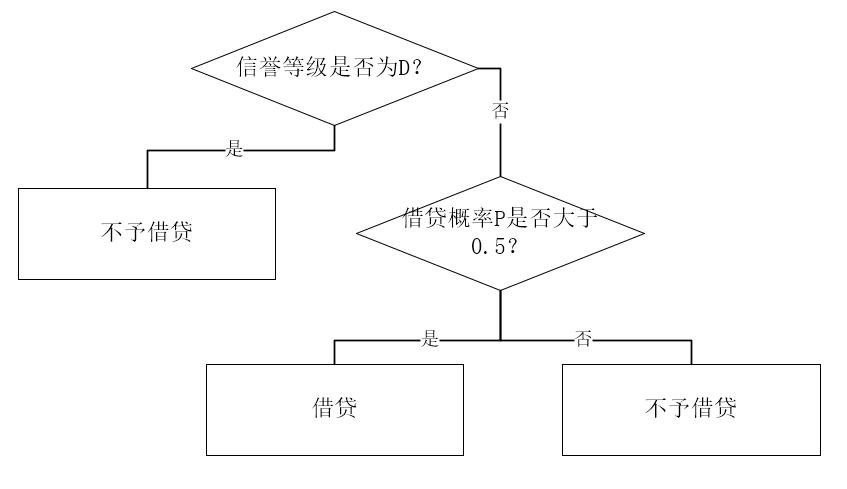
\includegraphics[width=0.8\textwidth]{511.png}
\caption{银行信贷判断图} % 标题
\label{five}
\end {figure}
\newpage
\subsubsection{贷款数量界定}
中小企业由于其经营策略的不同,需要周转的资金数量也有差异。界定中小企业的贷款需求,精准投放有限的资金储备,是银行需要解决的问题。在完成发放贷款与否的界定后,我们将使用熵权法来给出企业贷款数额的界定。

为了更好的判断借款数额,不仅需要利用式(\ref{x1}-\ref{x5})所定义的数值,还需要引入企业的资金缺口$x_6$作为附加的变量。企业在经营的过程中,遵循着先投入后产出的规律,只有首先购进材料产品等,随后售卖盈利,在这一过程中,存在一段时间企业投入资金大于收入所得。在这段时间内产生的支出与获利之差我们定义为资金缺口。当企业获得贷款能够补齐资金缺口时,便可以顺利保证经营的正常进行。我们记录资金缺口为:
\begin{equation}
    x_6 =\sum\limits_{t\in T\text{缺口进项}}t-\sum\limits_{t\in T\text{缺口销项}}t
\label{x6}
\end{equation}

对于许多小企业而言,需要使用同一套标准来计算其贷款额度。计算的依据是$x_1,\cdots,x_6$这六个指标,分别代表利润率,有效交易占比,供应链丰富度,信誉等级,平均单价,资金缺口六个要素。这六个要素量纲不同,数值不同,需要利用熵权法来给定各个因素在贷款分配策略中所占有的权重。其具体步骤如下:
\begin{enumerate}
    \item 利用附件中的数据,计算$i$用户($i=1,2,3,\cdots,m$)的$j$项指标$x_{ij}$($j=1,2,3,\cdots,6$)数值,构成用户指标矩阵$X_{m\times n}$,每项指标的计算方法如下:
    $$\begin{cases}
        x_1 = \frac{\sum\limits_{t\in T\text{销项}}t-\sum\limits_{t\in T\text{进项}}t}{\sum\limits_{t\in T\text{进项}}t}\\
        x_2 = \frac{card(T_{\text{有效},t>0})}{card(T)}
            \\
            x_3 = card(c_{\text{购方}})+card(c_{\text{销方}})
        \\x_4 = \begin{cases}
            1,A\\
            0.75,B\\
            0.5,C\\
            \text{不予放贷},D\\
        \end{cases}\\
        x_5 = \frac{\sum\limits_{t\in T\text{销项}}t+\sum\limits_{t\in T\text{进项}}t}{card(T_{\text{进项}})+card(T_{\text{销项}})}
        \\
        x_6 =\sum\limits_{t\in T\text{缺口进项}}t-\sum\limits_{t\in T\text{缺口销项}}t
\\
    \end{cases}$$

    \item 利用$X$,按照熵权法的步骤进行分配权重的计算。
    
   
    \begin{align}
    p_{ij} &= \frac{x_{ij}}{\sum\limits^n_{i=1}x_{ij}}\\
    \label{p}
    e_j &= -\frac{1}{\ln n}\sum\limits^n_{i=1}p_{ij}\\
    \label{ej}
    g_j &= 1-e_j\\
    % \label{gj}
    w_j &= \frac{g_i}{\sum\limits^m_{j=1}g_j}
    \label{dw}
    \end{align}
    式(\ref{p})利用各个指标出现的概率$p$计算熵值,并且在式(\ref{dw})中计算各项指标的权重$w_{ij}$。该方法由数据自身给出结果,较为客观有效。

    \item 利用得出的权重$w_j,j=1,2,\cdots,6$,可以计算每个企业的贷款评分数值$s$。
    \begin{equation}
    s_i = \sum\limits^m_{j=1}w_j\cdot x_{ij}
    \label{si}
    \end{equation}

    \item 在计算出每一企业的贷款评分数值$s_i$后,根据数值在当年贷款企业总评分$S$之间的占比来分配银行贷款总额$C_0$。
    \begin{equation}
    \begin{aligned}
        S &= \sum\limits^n_{i=1} s_i\\
        C_i &= C_0 \cdot \frac{s_1}{S}\\
    \end{aligned}
    \label{sci}
    \end{equation}
    至此,我们便计算出在有能力偿还贷款的企业中,各企业分配的贷款金额$C_i$。
\end{enumerate}

\subsubsection{贷款利率确定}
银行的贷款利率会影响客户的续借情况,过高的贷款利率给企业带来负担,最终导致企业不再继续向该行借款。这种不再续借的现象称为用户流失。银行要做到收益最大化,需要平衡利率和流失率之间的关系。

分析附件三中的数据,并做可视化,得到图(\ref{513}):
\begin {figure}[h]
\centering % 居中显示
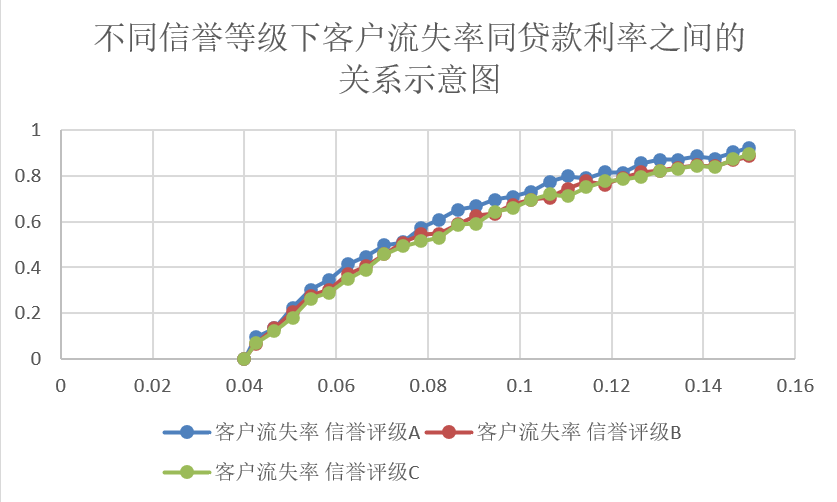
\includegraphics[width=\textwidth]{513.png}
% 标题
注:横轴代表贷款利率,纵轴代表用户流失率。
\caption{不同信誉等级下客户流失率同贷款利率之间的关系示意图} 
\label{513}
\end {figure}

可见当贷款利率上升时,用户流失率也随之上升,基本反映了客观规律。且横向对比不同信誉评级的客户,具有较高信誉评级的客户,面对同一借款利率是较容易流失的。这是由于信誉较好的企业能够在同等条件下获得更佳的利率优惠,银行承担的违约风险较小,因而面对较高的贷款利率时可以做出其他选择。

银行借贷的策略,不仅需要保证当期的贷款能够获得较高利润,还要确保未来还有稳定的客户来源,因此需要保持较低的流失率。为此,我们提出了一个兼顾二者的方法,将这一问题转换为多目标规划的问题。银行考虑取得最佳收益,这要求对每个用户都给出最佳的利率$I_i$,以兼顾收益和发展。

给出两个指标:信贷收益$R$和流失率$L$。
\begin{itemize}
    \item 信贷收益$R$
    
    即银行借款,按照利率$I$收回本息后,可以获得的利润。对于用户$i$而言,若其利率为$I_i$,银行贷款额度(5.1.2节)为$C_i$,则银行在该用户上的信贷收益$R$计算如下:
    \begin{equation}
    R_i = C_i\cdot I_i
    \label{r}
    \end{equation}
    \item 流失率$L$
    
    流失率定义为次年用户不再续借人数同当年借款人数的比例,其关于贷款利率和信誉等级的关系已经由附件三给出,可以使用拟合的方法给出关系式$f(I,grade)$来求解。
    \begin{equation}
    L_i = f(I_i,grade)
    \label{l}
    \end{equation}
\end{itemize}

为了综合考虑这两个指标,还需要对得到的数据做进一步处理,在计算出每个用户的信贷收益$R$和流失率$L$后,计算两个指标的最大值最小值,做归一化处理。
\begin{equation}
\begin{aligned}
    R_i^* &= \frac{R_i-R_{min}}{R_{max}-R_{min}} \\
    L_i^* &= \frac{L_i-L_{min}}{L_{max}-L_{min}} \\
\end{aligned}
\label{star}
\end{equation}
利用归一化后的指标,分别赋权,作为目标函数$F$:
\begin{equation}
\underset{I_i}{argmax}F = \omega_1 \cdot R_i^*+\omega_2 \cdot L_i^*
\label{}
\end{equation}
,其中$R_i^*$和$L_i^*$分别由式(\ref{r})式(\ref{l})以及式(\ref{star})得出,如下所示:
\begin{equation}
\begin{aligned}
    R_i^* &= \frac{C_i\cdot I_i-R_{min}}{R_{max}-R_{min}} \\
    L_i^* &= \frac{f(I_i,grade)-L_{min}}{L_{max}-L_{min}} \\
\end{aligned}
\label{}
\end{equation}
至此便得出针对每一用户的最佳利率。
\subsubsection{模型求解}
\subsection{没有借贷记录下的银行信贷模型}
对比附件一和附件二中数据,可以观察到附件二中的企业没有借贷记录,在数据上体现为缺失信誉评级$x_4$和违约记录。我们需要对其可能的信用评级进行预测。因此,我们不能直接使用5.1中建立的银行信贷模型,而需要先通过K近邻法\cite{6}对用户的信用评级进行预测,随后使用银行信贷模型组织信贷分配。

\subsubsection{基于K近邻算法的信誉评级预测}

K近邻算法是一种非参数的监督学习方法,其最大的特点是不需要训练。依赖已有的训练集数据进行投票,从而确定样本的类别。在前面的工作中,我们提出了一系列关于信贷偿还能力的指标,包括利润率,有效交易占比,供应链丰富度,平均单价等四个要素。一般而言,具有良好信用评级的企业都拥有相似的特质,每个企业的“特性”可以由一个四元向量$\vec{a}(x_1,x_2,x_3,x_5)$构成,各项分别代表利润率,有效交易占比,供应链丰富度,平均单价四个要素。

在得到企业经营特点的向量表示后,使用向量距离$d$来度量两个企业之间的相似度:
\begin{equation}
d = \left\lVert \vec{a}-\vec{b}\right\rVert 
\label{}
\end{equation}
,这里$\vec{a},\vec{b}$代表两个企业的特征向量,距离度量可以使用欧几里得距离,曼哈顿距离等,依据问题的不同来选定。

要对一个企业的信誉等级进行预测,可以由其周围$k$个最近的企业投票决定。如图(\ref{knn})所示:
\begin {figure}[h]
\centering % 居中显示
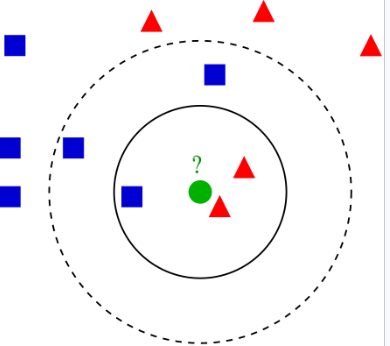
\includegraphics[width=0.6\textwidth]{521.png}

注:图中彩色物体代表企业特征向量在二维上的可视化示意图。红色代表信誉等级为A,蓝色表示信誉等级为B,绿色表示待归类的企业数据。(其余信誉等级企业未列出)
\caption{k近邻预测示意图} % 标题
\label{knn}
\end {figure}

\newpage
若取$k$值等于3,则记录信誉等级为A的票数为2,等级为B的票数为1,按少数服从多数的原则,待分类企业的信用等级为A。

依照上述步骤,可以对附件二中未知评级的企业数据依次进行处理,得到评级预测结果之后,使用银行信贷模型进行信贷资金分配。

\subsubsection{模型求解}

\subsection{企业行业类型的划分}
\subsubsection{企业行业类型的划分}
我们首先进行标准行业特征字、词的确定。通过对行业名称的观察和研究,我们发现企业名称能够很大程度上表明企业所在的行业。所以我们按照国民经济行业分类划分出16大类行业(鉴于医药业在疫情中有十分重要的地位,制造业分细分成了其他和医药制造业)。并依据国家行业标准\cite{7}等资料和文献将每类行业中企业名称的关键字和词提取出来。

在得到样本词和企业关键词后,我们将样本企业划分到所属的标准行业。因为能够表明企业所属行业的关键词均为1个和2个字的词语,所以我们只需将各企业的名称划分成单个字和两个相邻字为一组的词语,并将这些从企业名称中提取的字和词语与各行业的特征字、词进行匹配和对应,最终将该企业归到特征字、词重复数量最多的行业中。

\subsubsection{疫情对各类行业影响的确定}
    在划分企业类型后,我们进行受疫情影响的相关自变量的确定。经查阅相关资料和文献\cite{8,9},发现疫情对企业经济生产最重要的影响就在经营利润和资金缺口上。所以我们主要还会更改企业还款能力评估模型中的利润率和贷款数量界定模型中的年平均利润和投资资金缺口。

随后判断疫情对各行业影响程度。经过查阅新冠疫情对国民经济的影响等资料,我们得到了疫情对各类行业的影响程度,如表(\ref{label})所示。

\begin{table}[htb]
\centering
\caption{新冠病毒疫情对不同行业的影响程度}
\begin{tabular}{c|c|c}
    \toprule
    行业分类             & 受疫情影响程度 & 特征关键字、词                       \\
    \midrule
    农、林、牧、渔业         & 提高15\%  & 农、林、牧、渔                       \\
    采矿业              & 下降20\%  & 金属、材料、矿                       \\
    制造业(其他)          & 下降20\%  & 食品、饮料、酒、烟草、服饰、   \\
    &&家具、纸、汽车、电气、电器\\
    制造业(医药)          & 提高40\%  & 医药、医疗                         \\
    电力、热力、燃气及水生产和供应业 & 下降40\%  & 电力、热力、燃气、水                    \\
    建筑业              & 下降10\%  & 土木、房屋、建筑                      \\
    批发和零售业           & 下降20\%  & 批发零售                          \\
    交通运输、仓储和邮政业      & 下降20\%  & 物流、运输、邮政、交通                   \\
    住宿和餐饮业           & 下降40\%  & 住宿、餐饮                         \\
    信息传输、软件和信息技术服务业  & 提高30\%  & 电信、广播、网络、软件、信息、电子             \\
    金融业              & 提高20\%  & 货币、金融、资本、保险                   \\
    房地产业             & 下降21\%  & 地产、房产                         \\
    租赁和商务服务业         & 下降50\%  & 商业、服务、租赁                      \\
    教育               & 提高20\%  & 教育                            \\
    文化、体育和娱乐业        & 提高20\%  & 新闻、出版、广播、电视、电影、\\&&录音、文化、艺术、体育、娱乐\\
    \bottomrule
  \end{tabular}
\label{label}
  \end{table}

  \newpage
  \subsubsection{信贷策略的调整}
  设疫情对行业的影响程度为$\alpha$,规定其含义如下:
  $$\alpha\begin{cases}
    >0,\text{疫情有利于行业发展}\\
    <0,\text{疫情不利于行业发展}
  \end{cases}$$

  利用$\alpha$这个调整因子,将企业还款能力评估模型修改如下,对利润率$x_1$指标进行系数调整,其余保持不变。
  \begin{equation}
    \begin{aligned}
        P &= \frac{1}{1-\mathit{e}^{-Y}}\\
        Y &= \alpha + \beta_1x_1 +\beta_2x_2 +\beta_3x_3 +\beta_4x_4 +\beta_5x_5 \\
    \end{aligned}
\label{py2}
\end{equation}
$$\begin{cases}
    x_1 = \frac{\sum\limits_{t\in T\text{销项}}t-\sum\limits_{t\in T\text{进项}}t}{\sum\limits_{t\in T\text{进项}}t}\textcolor{red}{(1+\alpha)}\\
    x_2 = \frac{card(T_{\text{有效},t>0})}{card(T)}
        \\
        x_3 = card(c_{\text{购方}})+card(c_{\text{销方}})
    \\x_4 = \begin{cases}
        1,A\\
        0.75,B\\
        0.5,C\\
        \text{不予放贷},D\\
    \end{cases}\\
    x_5 = \frac{\sum\limits_{t\in T\text{销项}}t+\sum\limits_{t\in T\text{进项}}t}{card(T_{\text{进项}})+card(T_{\text{销项}})}
    \\
\end{cases}$$

随后对贷款数量界定模型进行修改,修改利润率$x_1$以及资金缺口$x_6$,其余保持不变。

\begin{equation}
    \begin{aligned}
        S &= \sum\limits^n_{i=1} s_i\\
        C_i &= C_0 \cdot \frac{s_1}{S}\\
    \end{aligned}
    \label{sci2}
    \end{equation}

    $$\begin{cases}
        x_1 = \frac{\sum\limits_{t\in T\text{销项}}t-\sum\limits_{t\in T\text{进项}}t}{\sum\limits_{t\in T\text{进项}}t}\textcolor{red}{(1+\alpha)}\\
        x_2 = \frac{card(T_{\text{有效},t>0})}{card(T)}
            \\
            x_3 = card(c_{\text{购方}})+card(c_{\text{销方}})
        \\x_4 = \begin{cases}
            1,A\\
            0.75,B\\
            0.5,C\\
            \text{不予放贷},D\\
        \end{cases}\\
        x_5 = \frac{\sum\limits_{t\in T\text{销项}}t+\sum\limits_{t\in T\text{进项}}t}{card(T_{\text{进项}})+card(T_{\text{销项}})}
        \\
        x_6 =(\sum\limits_{t\in T\text{缺口进项}}t-\sum\limits_{t\in T\text{缺口销项}}t)\cdot\textcolor{red}{(1+\alpha)}
    \\
    \end{cases}$$
\section{七、模型的评价}

\subsection{模型的优点}
\begin{enumerate}
    \item 此模型充分的利用了所给数据,并且对数据都进行了一定处理,将初始数据变为具有经济意义的指标。
    \item 企业还款能力模型采用多元线性回归,可以使各指标不仅与因变量P具有简单的线性关系,避免了线性拟合带来的弊端。
    \item 贷款数量的界定模型使用了熵权法,可以在没有储备相关知识的情况下做出客观的评价,提高了模型的适用性。
    \item 针对突发情况下的贷款策略调整模型仅在原有模型上进行修饰,可以整体上简化模型。
\end{enumerate}

\subsection{模型的缺点}
\begin{itemize}
    \item 突发情况下的贷款策略调整模型中对企业类型的划分可以使用更先进的文本聚类,但因时间有限未能完成,会降低模型的适用性。
\end{itemize}

%----------- 参考文献 ----------
\newpage
\begin{center}
\bibliography{reference} %调出LaTeX生成参考文献列表
\end{center}

%----------- 附录 ----------
\newpage
\section{附件}
\textbf{附件清单:}
\renewcommand\theenumi{\roman{enumi}}
% 规定数字格式为罗马数字
\renewcommand\labelenumi{\textbf{附录\theenumi}}
% 规定是附录某某
\begin{itemize}
    \item xxx代码
\end{itemize}

\textbf{sobel边缘检测代码}

\begin{lstlisting}[language=matlab]
    function GAdsa 
\end{lstlisting}



\end{document}